\documentclass[10pt]{article}
\newcommand{\HRule}{\rule{\linewidth}{0.5mm}}
\parindent 0pt
\parskip 10pt
\usepackage{anysize}
\usepackage{graphicx}
\usepackage{epsfig}
\usepackage{float}
%\usepackage{cite}
\usepackage{natbib}
\usepackage{setspace}
\marginsize{3.5cm}{3.5cm}{1cm}{1cm}
\onehalfspacing
\usepackage{caption}
\usepackage{subcaption}
\usepackage{amsmath,hyperref}

\usepackage{xcolor}
\hypersetup{
    colorlinks,
    linkcolor={red!50!black},
    citecolor={blue!50!black},
    urlcolor={blue!80!black}
}

%\textwidth 15cm
%\textheight 24cm
%\onehalfspacing
\begin{document}

\title{Bike Forecast}

\author{David Starkey}

\maketitle





\section{Introduction and Data Ingestion}
This project provides the details of bike hires in Montreal Canada dating from 2014 up to August 2017. The goal is to use statistical models to forecast the expected daily number of bike hires between two stations ( and ) for one weeks worth of hires between xxx and xxx. Each bike hire records the date, departure station and arrival station. This data is contained within several csv files which collectively total 15.3 million entries.

This summary is presented as follows. Section xx details the data ingestion process. Section xx presents the findings of the initial exploratory data analysis and includes several figures that motivate the model fitted to the global sample discussed in Section xxx. The results of the model fitting are provided in Section xxx.


\section{Data Ingestion}
\label{sec_ingest}



\section{Exploratory Data Analysis}
\label{sec_exp}

\subsection{Time Series}
Before deciding how best to model the forecasting problem, a universally sound first step is to visualise the data. I use Pythons matplotlib module to plot the number of bike hires as a time series, concatenating all four years of observations together. Figure \ref{fig_ts} presents some very important information on the Time Series

\begin{itemize}
\item The time series is periodic. It exhibits a similar annual pattern with bike hires becoming more popular in the summer months.

\item The amplitude of the variations appears to be increasing over time (smooth red line Figure \ref{fig_ts}). This suggests bike hires are increasing in popularity.
\end{itemize}




\begin{figure}
\begin{center}
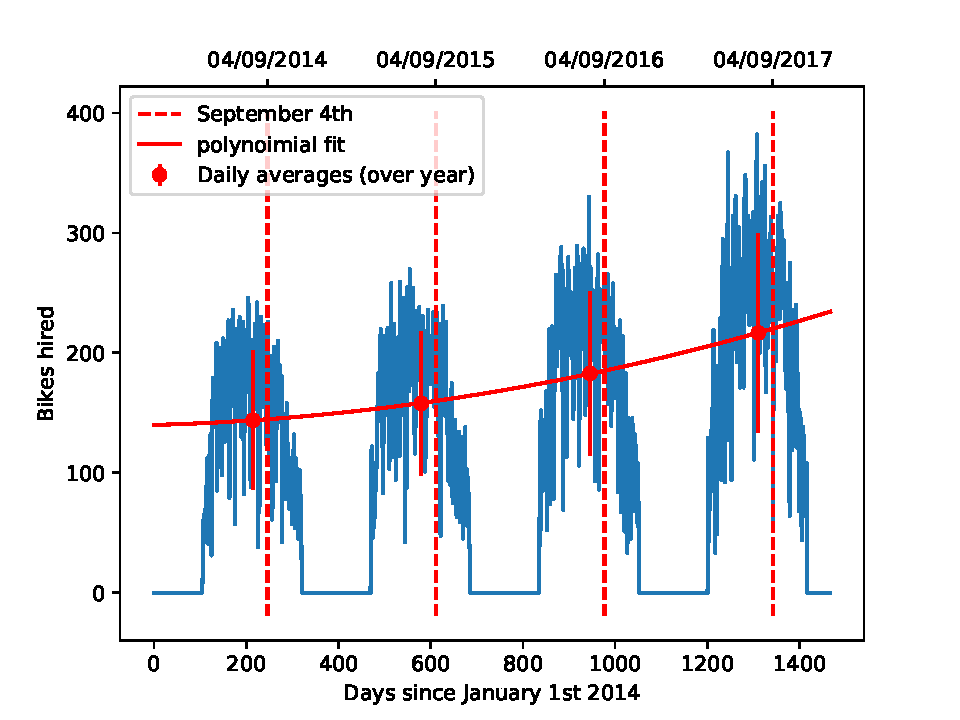
\includegraphics[scale=1.0,angle=0,trim=0cm 0cm 0cm 0cm]{ts_plot.pdf}
\caption{Time series of bike hires. Y axis plots the number of bikes hired per day as a function of day number (days are measured relative to 1st January 2014). The vertical red dashed lines show 4th September of each year (the start of the forecast week) and the smooth vertical polynomial fit shows how the average daily number of bike hires increases over the four years of data.}
\label{fig_ts}
\end{center}
\end{figure}
\begin{figure}
\begin{center}
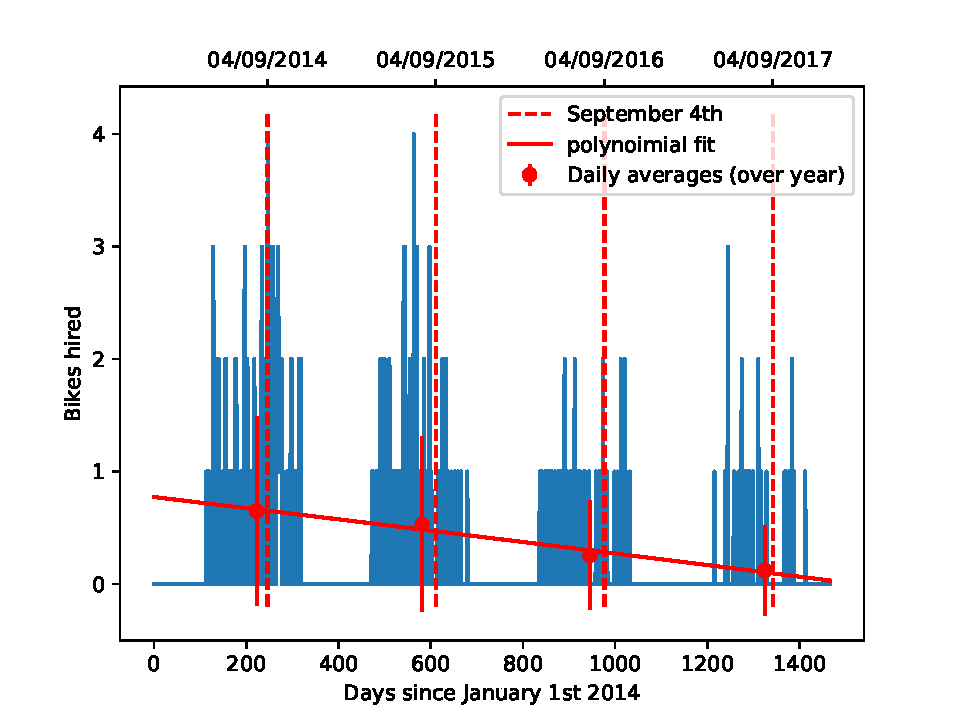
\includegraphics[scale=1.0,angle=0,trim=0cm 0cm 0cm 0cm]{ts_plot_station.pdf}
\caption{Same as Figure \ref{fig_ts} but restricting the time series only to bike hires departing at station xx and ending at station xx}
\label{fig_ts_station}
\end{center}
\end{figure}




While Figure \ref{fig_ts} provides useful information on the periodicity of the time series, this information is much clearer to see when presented as a power spectrum. The power spectrum as a function of frequency $P(f)$ can be computed from the fourier transform of time-series data $F(f)$ where

\begin{equation}
\label{eq_ft}
F(f) = \int_{-\infty}^{\infty} f(t) e^{-2\pi f t} dt,
\end{equation}
\noindent and $P(f)$ is then

\begin{equation}
\label{eq_ps}
P(f) = F^*(f) F(f),
\end{equation}

\noindent where $*$ denotes complex conjugation. Qualitatively, the power spectrum $P(f)$ tells us if there are strong periodic features in our data set. Figure \ref{fig_ps} demonstrates that the bike hires in this data set go through seasonal and weekly cycles of popularity, likely due to the seasonal weather / holiday season and weekend trend increases.





\begin{figure}
\begin{center}
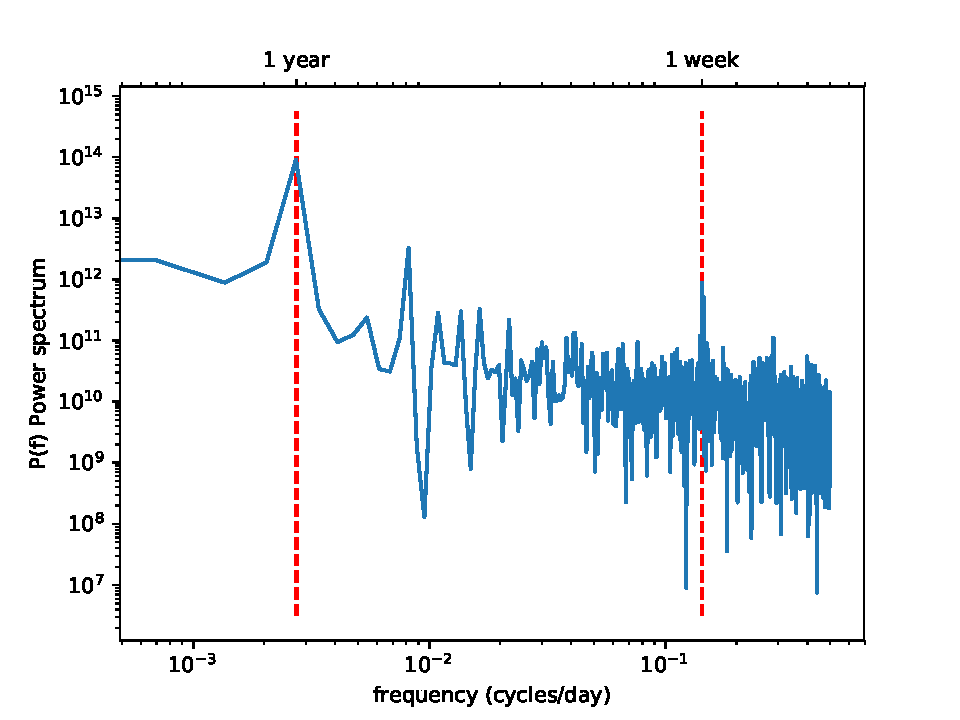
\includegraphics[scale=1.0,angle=0,trim=0cm 0cm 0cm 0cm]{ps_plot.pdf}
\caption{Power spectrum $P(f)$ versus frequency of the time series data presented in Figure \ref{fig_ts}. The peaks at one year and one week timescales (red dashed lines) show that bike hire goes through seasonal and weekly cycles of popularity.}
\label{fig_ps}
\end{center}
\end{figure}






\section{Model fitting (Auto Regressive Moving Average - ARMA)}
\label{sec_model}


Now that the periodicity of the bike hires is better understood, I will fit a model to the global sample to forecast the bike hires for the week beginning 4th September 2017. The model I use here is known as an Auto-Regressive-Moving-Average of ARMA model. AutoRegressive (the AR part) just means the model $Y(t_i)$ depends on the previous observation $Y(t_{i-1})$. The moving average part (MA) just means the process depends also on some unobserved quantity that we model as a draw from a Gaussian distribution. The numerical details of the model are outlined in Section \ref{sec_theory} but the reader is welcome to skip to the results in Section \ref{sec_results} if desired.


\subsection{Theory}
\label{sec_theory}
ARMA models are ideal for forecasting time series data and in general take the form

\begin{equation}
\label{eq_arma}
Y(t) = C + G(0,\sigma^2) + \sum_{i=1}^{p} A_i Y(t_{i-1}) + \sum_{i=1}^{p} B_i G(t_{i-1})
\end{equation}


\noindent where $C$ is the background level of the time series, $G(0,\sigma^2)$ indicates a draw from a Gaussian distribution with mean $0$ and variance $\sigma^2$. 


As with most optimisation problem, we want to find the best values of the parameters $\mathbf{\theta}$ that maximize a likelihood function $L( Y(t=1...T) | \mathbf{\theta})$, where the parameter vector $\mathbf{\theta}$ is explicitly given by

\begin{equation}
\mathbf{\theta} = \theta \left(C, \sigma^2 , A_{i=1,p}, B_{i=1,q}  \right),
\end{equation}

\noindent and the likelihood function $L( \mathbf{Y} | \mathbf{\theta})$. In general, one can optimize the parameters by differentiating a cost function (often $-2 \log L$ is used) with respect to each parameter and forming a `Hessian' Matrix $\underline{\underline{\mathbf{H}}}$ \footnote{Double underline here means a $N$ by $N$ matrix where $N$ is just the number of model parameters} out of the resulting system of equations such that.

\begin{equation}
\label{eq_hes}
\underline{\underline{\mathbf{H}}} \mathbf{\theta} = \mathbf{c(Y)},
\end{equation}
\noindent where $c(Y)$ is a constant vector dependent only on the observations $Y$, but not the parameters $\mathbf{\theta}$. The parameter vectors are then given by inverting this matrix and rearranging to form 
\begin{equation}
\label{eq_hespars}
\mathbf{\theta} = \underline{\underline{\mathbf{H}}}^{-1} \mathbf{c(Y)}.
\end{equation}

\noindent Depending on the order of the ARMA  process (the value $p$ and $q$), the model may be too complex to form a Hessian matrix and solve analytically. In this case here, numerical methods are used to optimize the parameters of the ARMA process used to fit the bike hire data. \footnote{Various texts exist for numerical optimization of ARMA  parameters (see for example \href{ http://www.phdeconomics.sssup.it/documents/Lesson12.pdf}{\textcolor{blue}{http://www.phdeconomics.sssup.it/documents/Lesson12.pdf}}).}








\section{Results}
\label{sec_results}
The ARMA model is trained on the history of bike hire time series observations (Figure \ref{fig_ts}) up to the 31st August 2017. The remaining entries in the csv file serve only as a bench mark test data set to test the models's accuracy. In Figures \ref{fig_arma_total} and \ref{fig_arma_zoom} , I first use the entire of the 2017 entries as the test data set to illustrate the predictive power of the ARMA model (in other words the model sees no data from 2017).


The objective is to forecast the number of trips between station ID 6184 and 6085. The ARMA model is now applied directly to the reduced sample and the results plotted in Figure \ref{fig_arma_station_total}. One issue here is that there are very few trips exclusively between these stations on which to base a forecast (only 340 in fact)


a sample restricted to entries between these stations (Figure \ref{fig_arma_station_total}) is that there are very few trips between these stations across all the years of data \footnote{The accompanying \verb|main_code.py| extracts these trips from all the csv files and saves them to a new file \verb|selected_station.csv|}. While it seems that the global trend is for the number of bike hires to be increasing with time (red smooth line Figure \ref{fig_ts}), the trips between stations 6184 and 6085 seem to have declined. The ARMA model applied to the restricted sample (340 trips) predicts no hires for the week starting 4th September 2017. While we see from Figure \ref{fig_arma_station_zoom} that this indeed proved to be true, we are not `supposed' to see this data and so would ideally like a second approach.

%One such method is to fit the ARMA model to the global sample and then reduce the model by a scaling function that evolves with time. This function to accurately model the relative fraction of the total sample that hires bike specifically between stations 6184 and 6085. The scaling function $S(t)$ can be derived from the yearly averages of global bike hires $\langle g \rangle (t)$ (smooth red line Figure \ref{fig_ts}), and yearly averages of bike hires from station 6184 and 6085 $\langle s \rangle (t)$ such that 

%\begin{equation}
%\label{eq_scale}
%S(t) = \langle s \rangle (t) / \langle g \rangle (t)
%\end{equation}


%\noindent The final expression for the forecasted hires $F(t)$ between Station 6184 and 6085 is then
%\begin{equation}
%\label{eq_scale_final}
%F(t) = S(t) Y(t).
%\end{equation}
%\noindent where $Y(t)$ is the ARMA model fitted to the global sample.


The resulting forecasts are outputed to the file xxx and Figure xxx below shows the results



\begin{figure}
\label{fig_arma_total}
\begin{center}
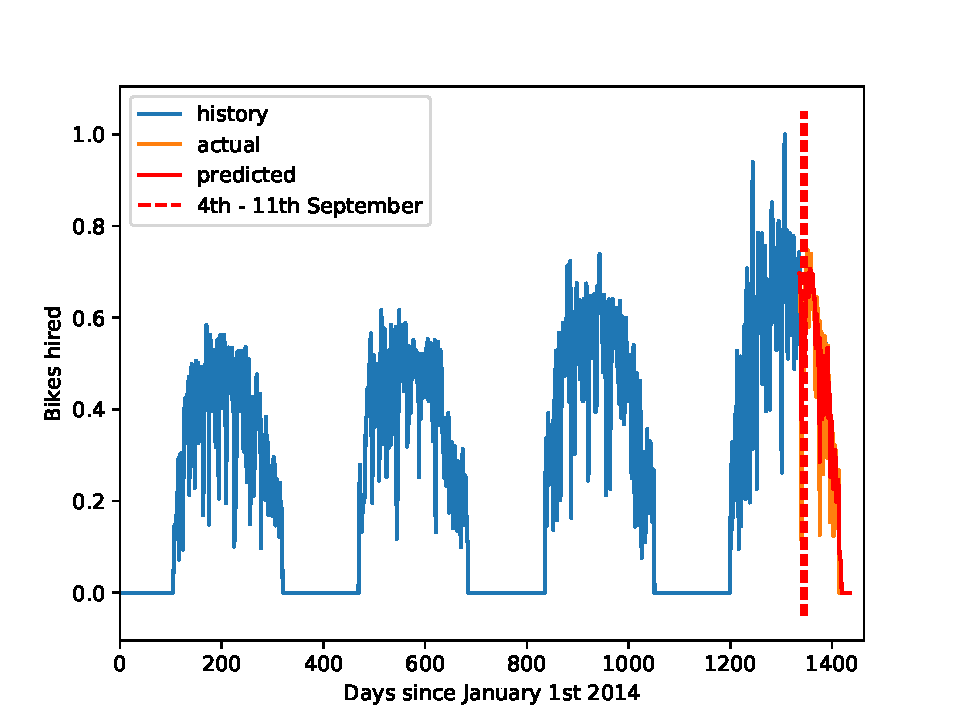
\includegraphics[scale=1.0,angle=0,trim=0cm 0cm 0cm 0cm]{arma_total_ts.pdf}
\caption{As with Figure \ref{fig_ts} but the red lines now show the ARMA forecast beyond the final training data point (31st August 2017). Dashed red lines enclose the requested forecast period (4th - 11th September).}
\end{figure}

\begin{figure}
\label{fig_arma_zoom}
\begin{center}
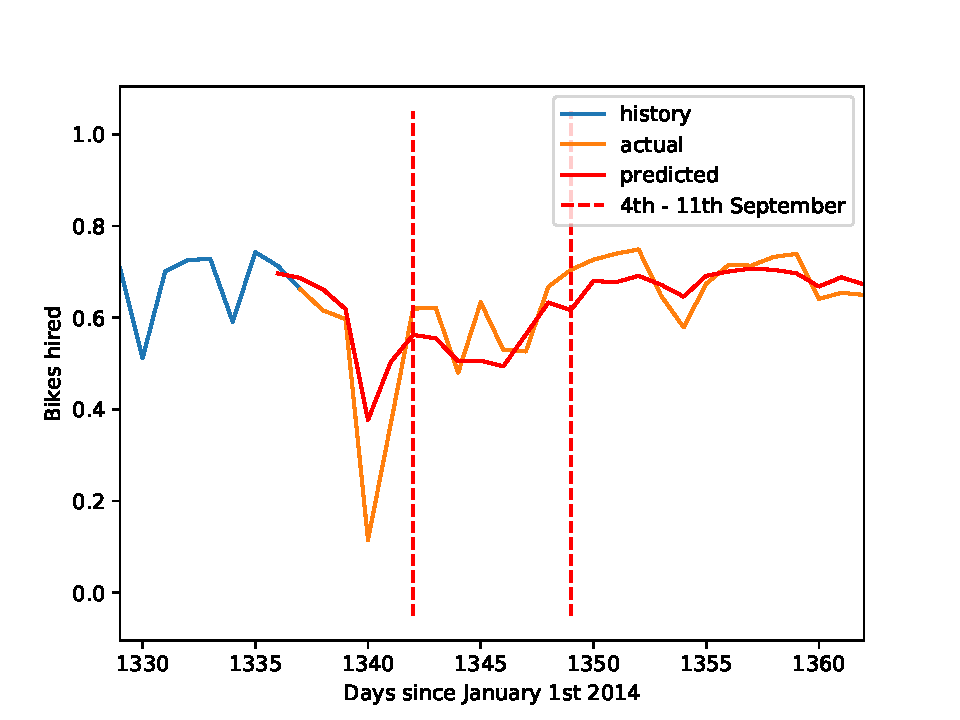
\includegraphics[scale=1.0,angle=0,trim=0cm 0cm 0cm 0cm]{arma_zoom_ts.pdf}
\caption{As with Figure \ref{fig_arma_total} but shwoing a zoom in of the requested forecast week (4th - 11th September).}
\end{figure}


\begin{figure}
\label{fig_arma_station_total}
\begin{center}
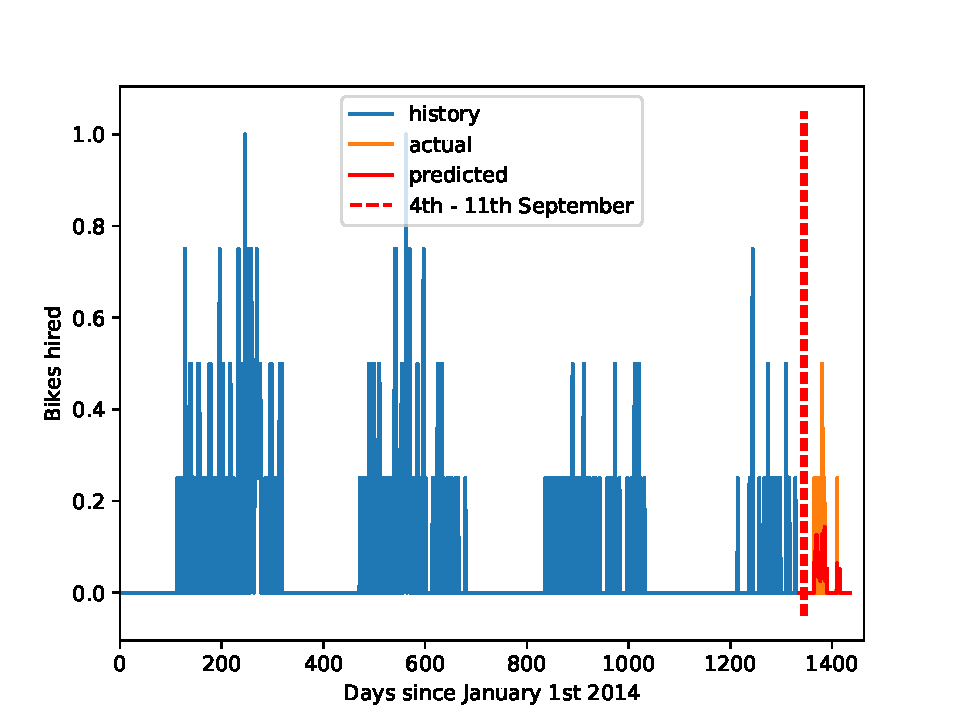
\includegraphics[scale=1.0,angle=0,trim=0cm 0cm 0cm 0cm]{arma_total_ts_station.pdf}
\caption{As with Figure \ref{fig_arma_total} but showing only the forecasts between station 6184 6085.}
\end{figure}

\begin{figure}
\label{fig_arma_station_zoom}
\begin{center}
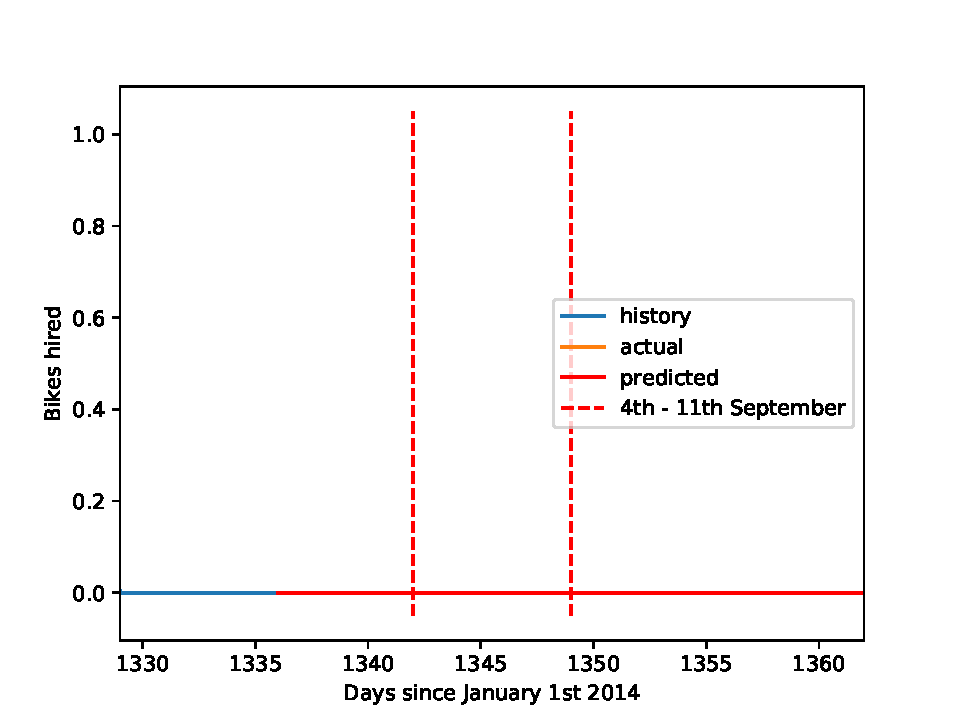
\includegraphics[scale=1.0,angle=0,trim=0cm 0cm 0cm 0cm]{arma_zoom_ts_station.pdf}
\caption{As with Figure \ref{fig_arma_station_total} but showing a zoom in of the requested forecast week (4th - 11th September).}
\end{figure}




\section{Conclusions}
I have used various python modules including Pandas, Numpy, Csv, Keras and Matplotlib to ingest several million entries of bike hires between various stations in Montreal. I have visualised these data to identify periodic trends affecting the frequency of hires using a power spectrum analysis. I then forecast the expected frequency of hires (trips per day) for 1 week starting 4th September 2017 to both the global sample and specifically between Stations 6184 and 6085.

The ARMA models fitted are ideal for time series analysis but a potential draw back of the model is the need to specify in advance the number of autoregressive coefficients (the $p$ number of previous time series points to consider) and the number of moving average $q$ coefficients. Including too few of these can restrict the model and prevent it from fitting high frequency features or long term behaviour. Fitting too many of these can lead to over-fitting problems. A good check of the appropriate number of parameters to include in these models would be some form of Bayesian model regularisation check like the Bayesian Information Criterion (BIC). This includes a penalty into the cost function for models with large number of parameters and introduces a trade-off between a well fitting model and a reasonably small number of parameters. Such a check could form the basis of future investigations.

Thanks you for taking the time to review this analysis. 




\end{document}